\chapter{Sprint 5: Implementing CI/CD}
In this final chapter, we will focus on Sprint 5, which is dedicated to implementing Continuous Integration and Continuous Deployment (CI/CD) for our project.

The objective of this sprint is to automate the build, test, and deployment processes to ensure efficient and reliable delivery of our application. Key components of this sprint include setting up GitHub webhooks, configuring the Jenkins pipeline, integrating SonarQube for code quality testing, containerizing the application, and deploying the containerized image to our Nexus private repository.


\pagebreak

\section{Analysis of Sprint 5 Requirements}
In this section, we will analyze the requirements for Sprint 5, focusing on the implementation of Continuous Integration and Continuous Deployment (CI/CD) for our project. This sprint involves setting up GitHub webhooks, configuring the Jenkins pipeline, integrating SonarQube for code quality testing, containerizing the application, and deploying the containerized image to our Nexus private repository. To illustrate these processes and provide a clear understanding of the interactions and workflows involved, we will use a BPMN (Business Process Model and Notation) diagram

\subsection{BPMN Diagram for our CI/CD Pipeline}

The following figure (\hyperref[fig:bpmn]{Figure \ref{fig:bpmn}})  represents the uses cases of our sprint.
\begin{figure}[h]
  \center
%\hspace*{-0.9in}
  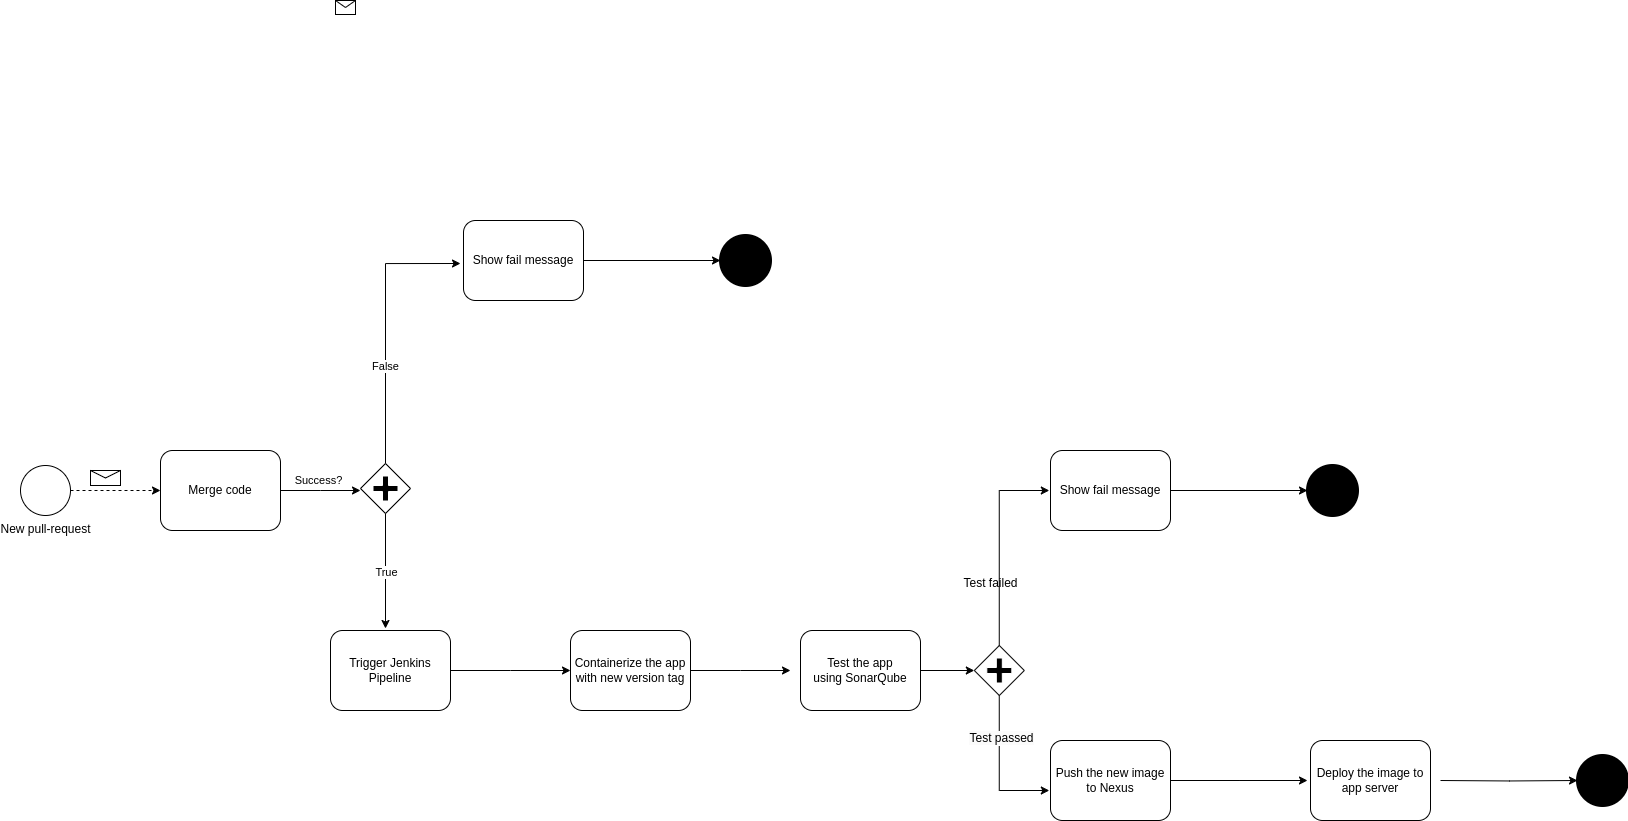
\includegraphics[width=17cm]{./chapters/sprint5/bpmn.png}
  \caption{BPMN Diagram}
  \label{fig:bpmn}
\end{figure}

\subsection{Interfaces}
In this section, we will provide screenshots and detailed explanations of the interfaces related to the CI/CD implementation as part of Sprint 5. These interfaces include Jenkins, GitHub webhook configuration, and SonarQube.

The following figure (\hyperref[fig:jenkins]{Figure \ref{fig:jenkins}})  depicts the Jenkins server interface.
Jenkins is used to automate the build, test, and deployment processes. The Jenkins interface allows developers to create and manage CI/CD pipelines.
\begin{figure}[h]
  \center
%\hspace*{-0.9in}
  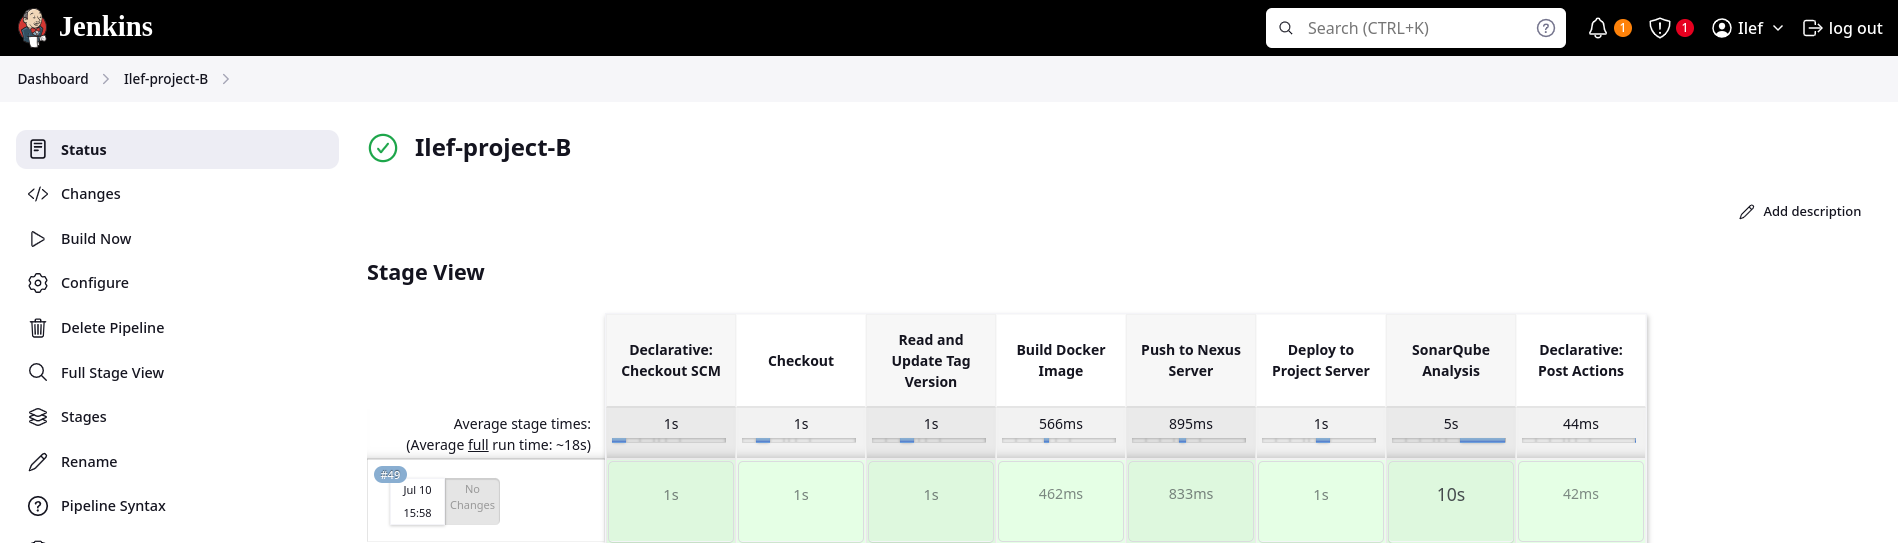
\includegraphics[width=14cm]{./chapters/sprint5/jenkins.png}
  \caption{Jenkins server interface}
  \label{fig:jenkins}
\end{figure}

The following figure (\hyperref[fig:jenkins]{Figure \ref{fig:jenkins}})  represents the SonarQube server interface.
SonarQube is integrated with Jenkins to perform static code analysis and ensure code quality.
\begin{figure}[h]
  \center
%\hspace*{-0.9in}
  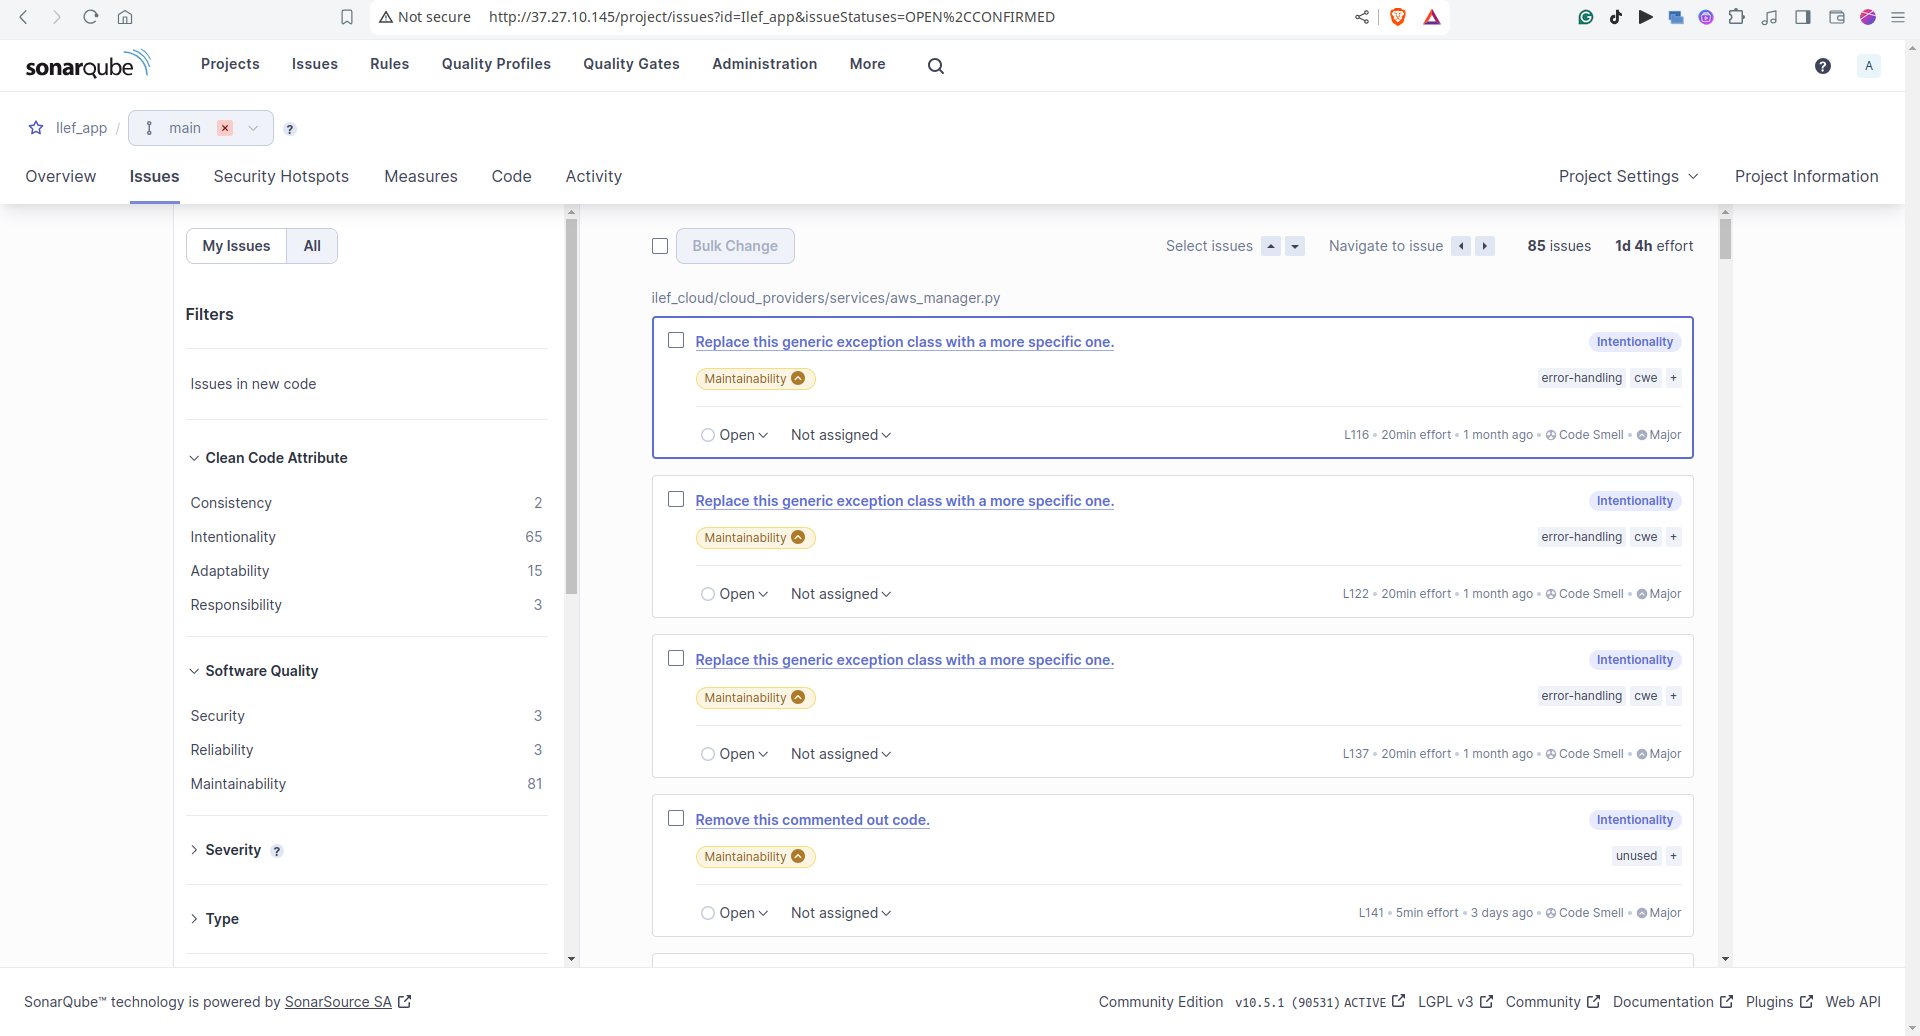
\includegraphics[width=14cm]{./chapters/sprint5/sonnar.png}
  \caption{Sonar server interface}
  \label{fig:jenkins}
\end{figure}

The following figure (\hyperref[fig:webhook]{Figure \ref{fig:jenkins}})  represents the GitHub Webhooks interface.
GitHub webhooks are used to trigger Jenkins jobs automatically when changes are pushed to the repository.
\begin{figure}[h]
  \center
%\hspace*{-0.9in}
  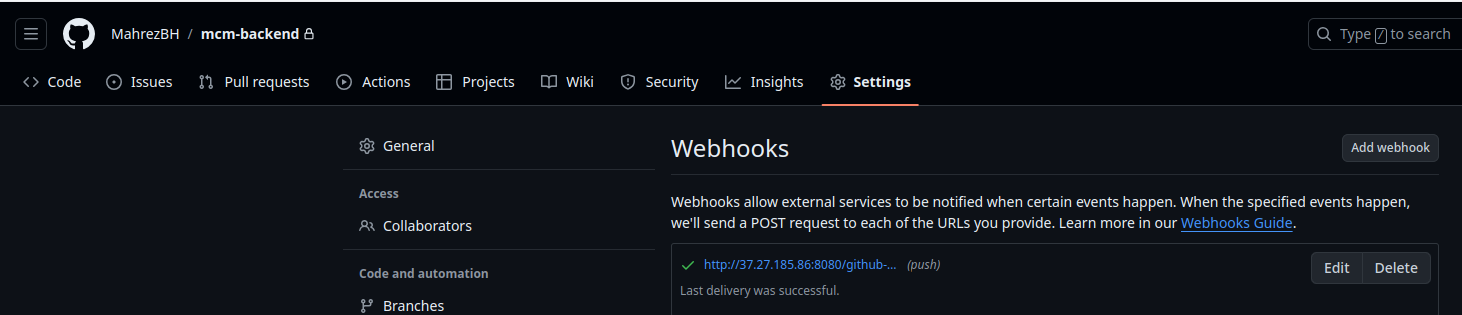
\includegraphics[width=14cm]{./chapters/sprint5/webhook.png}
  \caption{GitHub Webhooks interface}
  \label{fig:jenkins}
\end{figure}

\section*{Conclusion}
In this final chapter, we focused on Sprint 5, which was dedicated to implementing Continuous Integration and Continuous Deployment (CI/CD) for our project. We detailed the setup of GitHub webhooks, the configuration of the Jenkins pipeline, the integration of SonarQube for code quality testing, the containerization of the application, and the deployment of the containerized image to our Nexus private repository.

We illustrated these processes with a BPMN diagram to provide a clear understanding of the interactions and workflows involved. Additionally, we explored the interfaces of Jenkins, GitHub webhook configuration, and SonarQube, which are crucial for automating and managing the CI/CD pipeline.

By completing Sprint 5, we have significantly enhanced our development workflow, ensuring rapid, reliable, and high-quality software delivery. The implementation of a robust CI/CD pipeline establishes a strong foundation for continuous integration and deployment, improving our project's overall efficiency and stability.
\chapter*{General conclusion}

Cloud computing and container management are pivotal in modern information technology. Handling large volumes of data and deploying applications efficiently across multiple cloud providers can be challenging. Establishing a robust and scalable solution for cloud resource management is essential for ensuring optimal performance and productivity.

In this report, we presented the project's general context, outlined the problematic, examined current solutions, and proposed our innovative solution. We conducted a thorough preliminary study, covering basic concepts, requirements analysis, use case specifications, mockups, product backlog, logical and physical architecture, and the technologies to be used.

Throughout the implementation phase, we systematically developed and integrated various functionalities, including user management, instance and storage management, container management, data visualization, project management, and a CI/CD pipeline. Each phase was meticulously planned and executed, enhancing our application's capabilities and performance.

This project has been an enriching experience, significantly bolstering my technical skills and providing practical application of academic knowledge. Working within a collaborative and skilled team has also honed my soft skills.

In conclusion, this project has established a solid foundation for efficient cloud resource management, leveraging advanced technologies and best practices. The methodologies and solutions developed will serve as valuable assets for future projects, enabling the delivery of high-quality software solutions effectively and reliably.